%!TEX root=../../../template.tex
\subsection{Testing the Lambertian Hypothesis}%
\label{sub:methods_experiment}

The experiment involved two different optical assemblies, which are
summarised in Table~\ref{tab:assemblies}. Both assemblies play two
roles, which reflect the comparison between active and passive that is
the entire aim of the test. To simplify, we will address the two as West
Bank and East Bank. The West Bank is, as the name implies, the assembly
that is placed further West, i.e., the one that is installed on
\gls{iep}'s roof. By exclusion, the East Bank assembly is the one placed
on the sanctuary. The West Bank assembly is comprised of a telescope and
tripod, a spectrometer (with the necessary fibre optics attached) and a
laptop. 

The East Bank assembly has exactly the same parts, but in addition to
them, it features a hand-held torch that sports an XHP50.2 CREE LED. The
manufacturer states that this torch is capable of illuminating by itself
up to a distance of 300 m and produces luminous flux of at least 1500
lm. By fitting this torch on the telescope's eyepiece channel, we are
able to further collimate the light that it produces, making it reach
much further distances than originally stated, and being easily picked
up by the other telescope. This is plain to see in
Figure~\ref{fig:light_at_the_distance}. The light spectrum that pertains
to the CREE LED in use is published in this device's datasheet, and
presented in Figure~\ref{fig:cree_spectrum}, which largely corroborates
the spectrum in Figure~\ref{fig:measured_led_spectrum}, taken by the
same spectrometers that were used in the experiment, at a distance of
approximately 50 m from the torchlight. 

\begin{figure}[htpb]
    \begin{minipage}{.45\textwidth}
        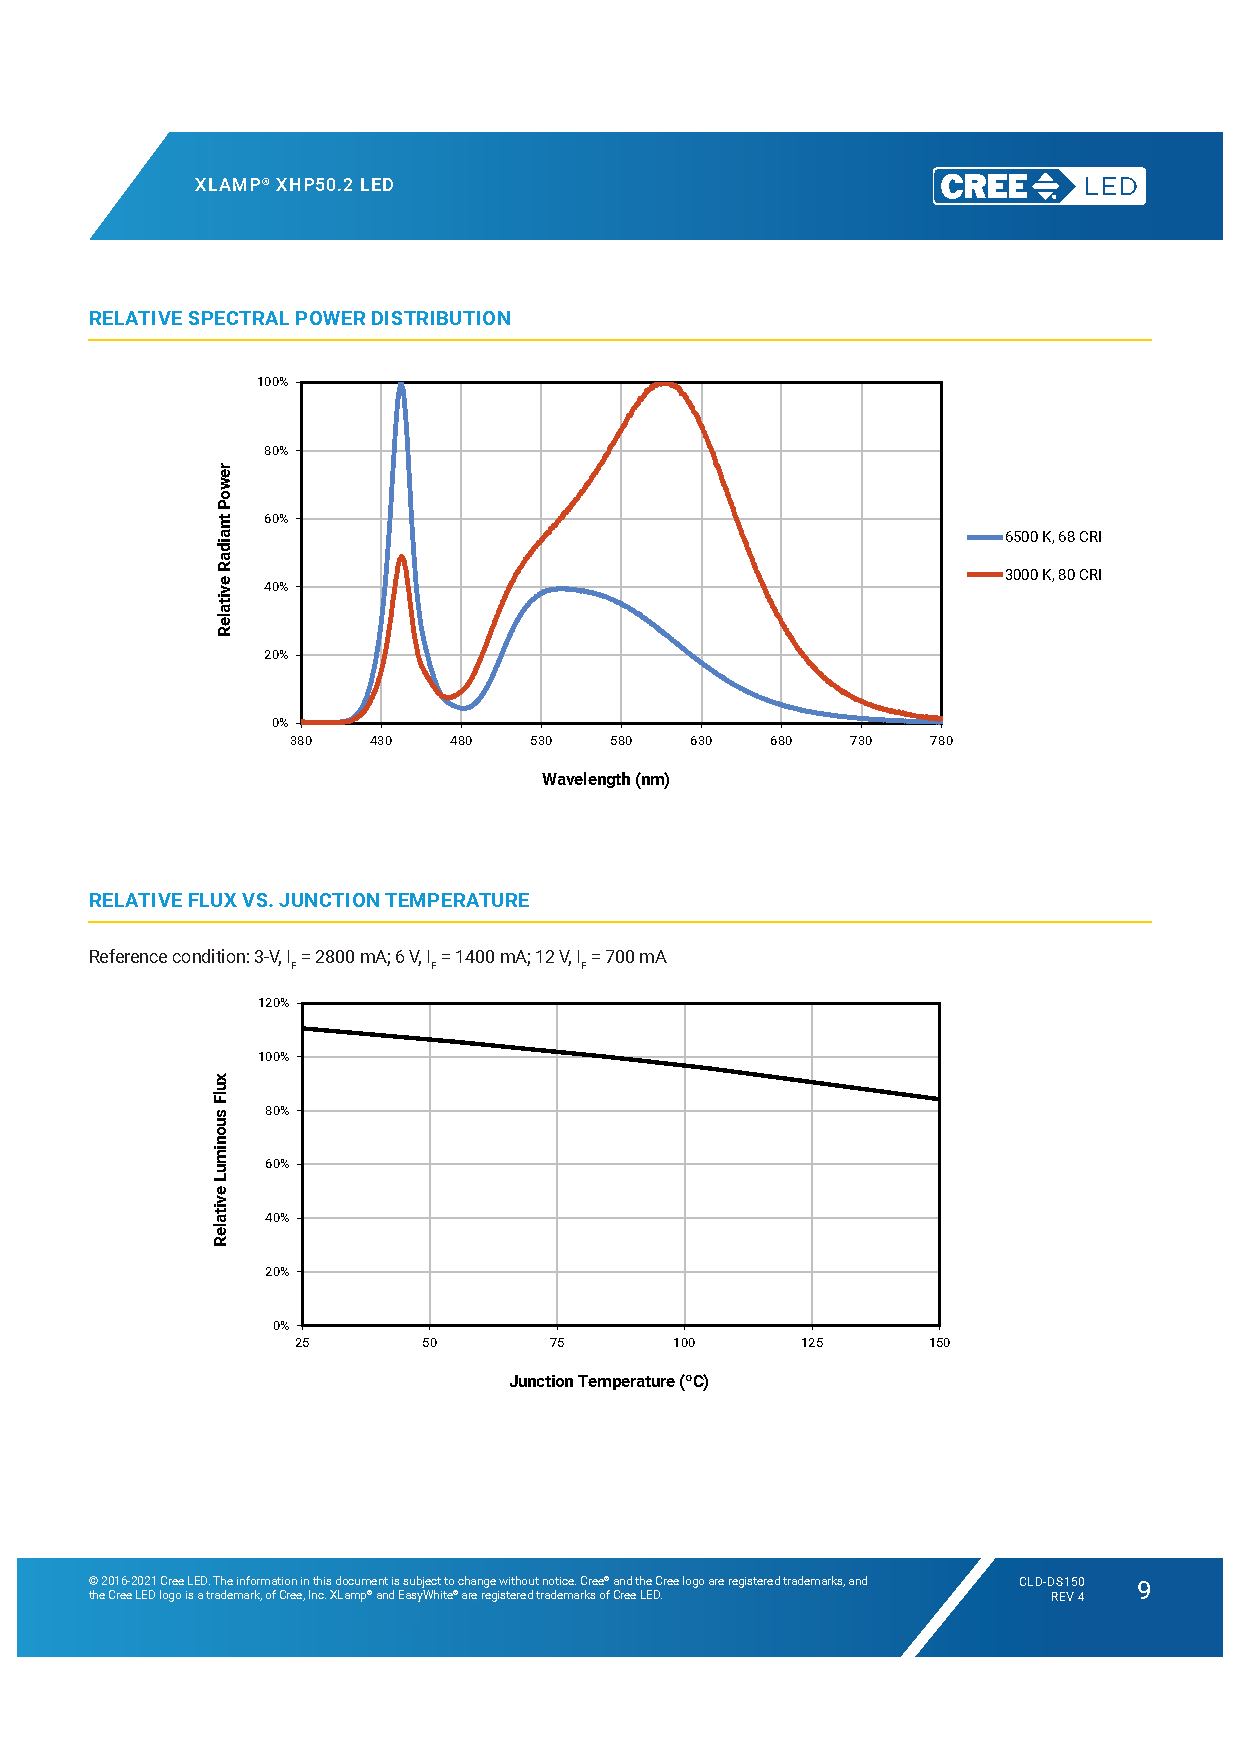
\includegraphics[trim=3cm 15cm 5cm 6cm, % ...
            clip, width=\textwidth]{img/pdf/cree_datasheet.pdf}
        \caption{Published spectrum of the CREE XHP50.2 LED
        light. The LED that was used in this
        experiment corresponds to the blue line~\cite{CREE2021}.}
        \label{fig:cree_spectrum}
    \end{minipage}
    \hfill
    \begin{minipage}{.45\textwidth}
        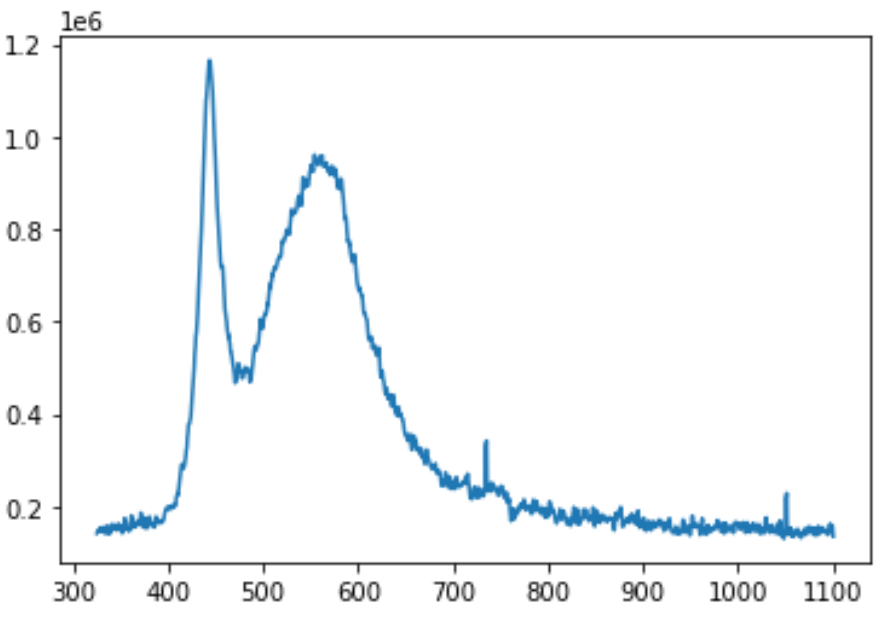
\includegraphics[width=\textwidth]{img/png/measured_led_spectrum.png}
        \caption{Spectrum measured with the experiment spectrometers, at
        a distance of approximately 50 m from the torchlight.}
        \label{fig:measured_led_spectrum}
    \end{minipage}
\end{figure}

\begin{table}[htpb]
    \centering
    \caption{Summary table for the two experiment assemblies. Note the
    difference in terms of material, due to the two different roles both
    assemblies play during the experiment. This is translated into not
    having the need of an artificial light source in the West Bank's
    assembly.}
    \label{tab:assemblies}
    \resizebox{\textwidth}{!}{%
        \begin{tabular}{@{}lll@{}}
            \toprule
            \textbf{} & \textbf{West Bank} & \textbf{East Bank} \\ \midrule
            \textbf{Spectrometer} & Avantes USB 2048 channels & Avantes USB 2048 channels \\
            \textbf{Telescope} & Meade ET90 & Meade ET90 \\
            \textbf{Artificial Light Source} & N/A & Goobay CREE XHP50.2 torch \\
            \textbf{Laptop} & Windows 10 laptop & Windows 10 laptop \\
            \textbf{Software} & AvaSoft 8.11 & AvaSoft 8.11 \\ \bottomrule
        \end{tabular}%
    }
\end{table}

The experiment itself is scheduled to start at around 06:00 A.M.. It
consists in capturing spectral measurements in both modes (active and
passive) periodically, with the least amount of time possible between
measurements in the same capture. In this case, I am calling capture to
a particular group of actions that are defined in
Table~\ref{tab:actions}. Captures are defined according to the time at
which they are run, and are summarised in Table~\ref{tab:captures}.
Closing time for this experiment was set on 11:00 A.M.. This time window
ensures measurements are taken during sunrise and until after the
morning rush hour is over.

\begin{table}[htpb]
    \centering
    \small
    \caption{Actions are the indivisible unit upon which each capture is
    built. The prescribed actions for this experiment are described in
    this table.}
    \label{tab:actions}
    \begin{tabularx}{\textwidth}{cXX}
        \toprule
        \textbf{Action ID} & \textbf{Action} & \textbf{Description} \\ \midrule
        A & Active trace gas concentration determination & With the two
        telescopes facing each other, we collect spectra for two minutes
        with the light source turned off and another 2 min with the light
        source turned on. \\
        \midrule
        B & Passive trace gas concentration determination & With the two
        telescopes aligned and approximately facing West, we collect spectra
        for 2 minutes. \\
        \midrule
        C & Passive reference collection & The West telescope points upwards
        and collects data for 2 minutes. \\ \bottomrule
    \end{tabularx}
\end{table}

\begin{table}[htpb]
    \centering
    \caption{Captures are particular sets of actions that are conducted
    according to a specific order, depending on the time of day on which
    the capture is run. This table describes the prescribed captures on
    which this experiment consisted.}
    \label{tab:captures}
    \begin{tabular}{@{}ccc@{}}
        \toprule
        \textbf{Time Frame} & \textbf{Period} & \textbf{Action} \\
        \midrule
        05:00 - Sunrise & 15 minutes & A \\
        Sunrise & Once & C \\
        Sunrise - 11:00 & 15 minutes & A and B\\
        \bottomrule
    \end{tabular}
\end{table}

As displayed in Table~\ref{tab:assemblies}, the spectrometers are both
the same model, manufactured by Avantes and with 2048 channels, powered
through the same \gls{usb} cable that is used for data transfer. The
spectra are acquired through Avantes' own collection software, AvaSoft
8. The spectrometer are configured to have an integration time of 20ms
and immediately store every measurement on an \gls{ascii} file. With the
kind of lighting conditions that we are dealing with, this integration
time allows us not to worry about saturation. However, to build usable
spectra we need to sum the collected files. This is valid because given
the very little time it takes to make a measurement (2 minutes), the sun
can be considered a constant light source, and therefore
we can consider the photons to have a Poissonian statistic
distribution~\cite{Fox2006}.




